\begin{chapter}{\label{cha:numerics}Numerical Algorithms}
\section{\label{section:RK} Numerical procedures for 2D and 3D solutions}
	\subsection{\label{section:RK4} Fourth order Runge-Kutta scheme}
	The classical fourth-order Runge-Kutta formula (RK4) is described equivalently in many texts. We follow the description in \cite{NumericalRecipes}. Let an initial value problem be specified as
	
	\begin{align*}
		\frac{\partial \psi}{\partial t} &= f(\psi,t),\hspace{0.25in}\psi(t_0) = \psi_0.
	\end{align*}

A step-size, $h>0$, is chosen as the parameter controlling how the solution is advanced over $t$. The scheme for estimating $\psi(t_n)= \psi_n$ is then written
\begin{equation}
\begin{split}
		k_1 &= hf(t_n,\psi_n),\\
		k_2 &= hf(t_n+\frac{h}{2},\psi_n+\frac{k_1}{2}),\\
		k_3 &= hf(t_n+\frac{h}{2},\psi_n+\frac{k_2}{2}),\\
		k_4 &= hf(t_n+h,\psi_n+k_3),\\
		\psi_{n+1} &= \psi_n + \frac{k_1}{6}+ \frac{k_2}{3}+ \frac{k_3}{3} + \frac{k_4}{6} + O(h^5),\\
		t_{n+1}  &= t_n + h.
		\label{eq:rk4}
\end{split}
\end{equation}


	A full derivation and proof of accuracy for the RK4 scheme is outlined in Appendix \ref{appsection:rk4deriv}.
	In all of our relevant calculations the value of f is set as the right hand side of the homogeneous or trapped GPE. The main loop formulating the RK4 method may be repeated indefinitely to reach any $t>t_0$. The step size for a given set of parameters should be chosen small enough that smaller choices make no quantitative changes to the resulting solution.

	\subsection{\label{section:numericalParams} Numerical stability}
	We now systematically study the numerical stability of common simulated systems. Our aim is to find a suitable discretisaton of space and time so that while simulations are timely, our numerical solutions are converged and not overly sensitive to small changes computational parameters.

	We use energy to measure because in the undamped gpe energy is conserved.

	We run 100 units of imaginary time stepping to get density profile
	We run another 100 units for vortex IC
	We run 500 units in real time to study stability


\begin{figure}
	\centering
	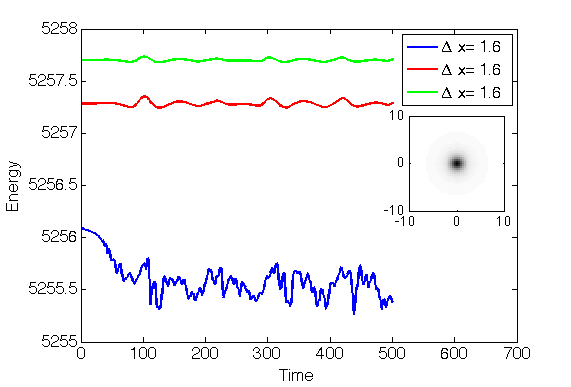
\includegraphics[width=0.5\textwidth]{numerics/figures/homg_energy_cons.png}
\end{figure}

\section{\label{section:vortexidentifying} Identifying vortices}


\subsection{\label{section:gaussianblur} Image filters and the Gaussian kernel}

\section{\label{section:vortexclustering} Quantifying vortex clustering}
	\subsection{\label{section:reevesalgorithm} Recursive Cluster Algorithm (RCA) }
		


	\subsection{\label{section:ripleysk} Ripley's K function }
		\begin{equation}\label{eq:ripleysk}
		K(x) = \frac{A}{n^2}\sum\limits_{i \ne j} I\left (d_{ij}<x\right ),
		\end{equation}
		where $d_{ij}$ is the distance between the $i$th and $j$th points, $A$ is the area of the region containing every point, $n$ is the number of points, $x$ is the search radius, and I is the indicator function (1 if its argument is true, 0 otherwise). Should the points be distributed homogeneously in space, then $K(s)\approx\pi s^2$.
\section{\label{section:vortextracking} Tracking vortex trajectories}
\section{\label{section:vortexremoval} Removing vortices with phase unwrapping}
	

\end{chapter}
